\documentclass[a4paper,10pt]{article}

%A Few Useful Packages
\usepackage{marvosym}
\usepackage{url,parskip}			%formatting
\usepackage[utf8]{inputenc} 
\usepackage{multirow}

%Graphics - Colors
\RequirePackage{color,graphicx}
\usepackage[usenames,dvipsnames]{xcolor}
% %better formatting of the A4 page
\usepackage[big]{layaureo}
%An alternative to Layaureo can be usepackage{fullpage}
 
\usepackage{supertabular} 		%for Grades
\usepackage{titlesec}			%custom section
 
%Setup hyperref package, and colours for links
\usepackage{hyperref}
\definecolor{linkcolour}{rgb}{0,0.2,0.6}
\hypersetup{colorlinks,breaklinks, urlcolor=linkcolour, linkcolor=linkcolour}

% \pagestyle{empty} % non-numbered pages
\usepackage[english]{babel}
\usepackage{slantsc}
\usepackage{array}
\usepackage{amsmath}

%FONTS
\usepackage[T1]{fontenc}
%\usepackage{arev}
%\newcommand{\fancyfont}{\fontfamily{avec}\selectfont}

%CV Sections inspired by:
%http://stefano.italians.nl/archives/26
\titleformat{\section}{\Large\scshape\raggedright}{}{0em}{}[\titlerule]
\titlespacing{\section}{0pt}{3pt}{3pt}

%XeTeX
%\usepackage{fontspec}			%load fonts
%\usepackage{xunicode,xltxtra} 	%other packages for XeTeX
%\defaultfontfeatures{Mapping=tex-text}
%\setmainfont[SmallCapsFont = Fontin SmallCaps]{Fontin}


%workEntry(end time, start time, job position, company, description)
\newcommand{\workEntry}[5]{
\begin{tabular}{p{1.7cm}|p{11cm}}
\raggedleft \textsc{#1} & #3 \\
\raggedleft \textsc{#2} & \emph{#4} \\
& \footnotesize{#5}\\
\multicolumn{2}{c}{}\ %this clears the space between two jobs
%some other job here
\end{tabular}
}

\newcommand{\dateEntry}[4]{
\begin{tabular}{p{1.7cm}|p{11cm}}
\raggedleft \textsc{#1} & #3 \\
\raggedleft \textsc{#2} & \footnotesize{#4}\\
\multicolumn{2}{c}{}\ %this clears the space between two jobs
%some other job here
\end{tabular}
}

\newcommand{\resEntry}[1]{
\begin{tabular}{p{1.7cm}|p{11cm}}
& #1 \\
\multicolumn{2}{c}{}\
\end{tabular}
}

\newcommand{\resEntryD}[2]{
\begin{tabular}{p{1.7cm}|p{11cm}}
& #1 \\
& \emph{#2} \\
\multicolumn{2}{c}{}\
\end{tabular}
}

\begin{document}

\par{\centering
{\huge{\textsc{Mart\'in A. Miguel}} }
\bigskip\par}

%Section: Personal Data
\section{Información Personal}
\begin{tabular}[c]{rp{7.5cm}r}
\textsc{Fecha de Nacimiento:} & 10 de Junio de 1990 & \multirow{4}{*}{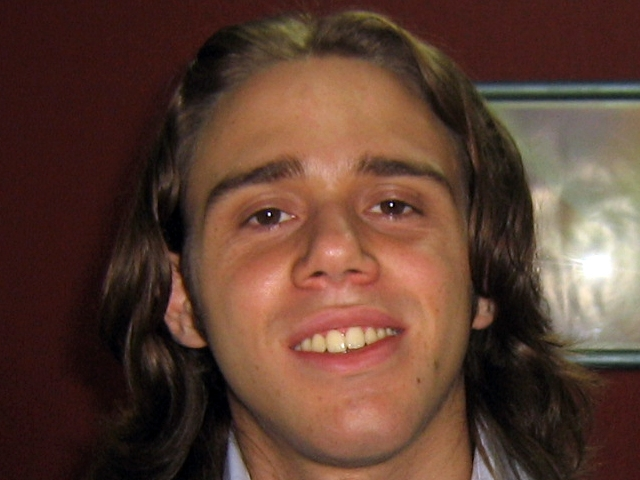
\includegraphics[scale=0.17]{../MMiguel-foto.jpeg}}\\
\textsc{Ubicación:}	& Almagro, Capital Federal, \newline Buenos Aires, Argentina & \\
\textsc{Teléfono:}	& 4983-4768 15-3181-6018 & \\
\textsc{email:}	& \href{mailto:m2.march@gmail.com}{m2.march@gmail.com} & \\

\end{tabular}

%Section: Objective
\section{Objetivo}
Mi búsqueda profesional actual se enfoca en el desarrollo de mis habilidades personales. Me interesa poner a prueba mis capacidades para enfrentar distintos tipos de situaciones que involucren tanto desafíos técnicos como profesionales. Deseo poder contribuir en proyectos, en particular aquellos que posean una cuota de desarrollo creativo, de forma de dar uso al conocimiento y la experiencia que adquirí durante mis estudios y carrera.
%My current professional objective focuses on the development of my personal skills. I am interested in testing my capability to face different types of situations, involving both technical and personal challenges. I look forward to contributing in projects, specially those where creative development is required, giving use to the knowledge and experience acquired throughout my studies and career.

%Section: Profile
\section{Perfil Profesional/Personal}
\begin{itemize}
 \item Analítico, buscador de lo eficiente %Analytical, efficiency-seeker
 \item Metódico, confiable %Methodical, reliable 
 \item Curioso, investigador e innovador %Curious, investigator, innovator
 \item Afable, considerado %Well-mannered, affable, thoughtful
\end{itemize}

%Section: Work Experience
\section{Experiencia laboral}
\workEntry{Presente}{Agosto 2012}{Programador Java}{Despegar.com}{}

\workEntry{Julio 2012}{Marzo 2012}{Docente Ayudante en la Carrera de Cs. de la Computación de la UBA}{Algoritmos y Estructuras de Datos I}{}

\workEntry{Diciembre 2011}{Marzo 2011}{Docente Ayudante en la Carrera de Cs. de la Computación de la UBA}{Algoritmos y Estructuras de Datos II}{}

\workEntry{Enero 2010}{Enero 2009}{Programador Java Jr. (J2ME / Blackberry)}{SenseByte}{}


%Section: Education
\section{Educación}
\workEntry{2012}{2009}{Lic. en Ciencias de la Computación}{Universidad de Buenos Aires - FCEyN}%
{15 materias finalizadas}

%\dateEntry{2008}{}{Ciclo b�sico com�n (CBC)}%
%{Finished}

\workEntry{2007}{2003}{Secundario con orientación en comunicaciones}{Instituto SUMMA}{}

\section{Inglés - Nivel Avanzado}
\workEntry{2006}{}{FCE - First Certificate in English}{AACI}{Grade A\newline
\hspace*{0.15cm} \emph{University of Cambridge, ESOL Examinations}}

\workEntry{2004}{}{CILE 3 - English Certificate}{Facultad de Filosof\'ia y Letras, UBA}%
{Score: 80/100}

\section{Conocimientos Técnicos}
\resEntry{Experiencia en los siguientes lenguajes: C, C++, Java, Groovy, Python, Intel x86 Assembler, Haskell, ActionScript 2.0}{}

\resEntry{Capacidades de uso de las siguientes tecnologías: LaTeX, Octave}{}

\resEntry{Experiencia en herramientas de diseño gráfico y web: Adobe Photoshop, Adobe Flash}{}

\resEntry{Uso de sistemas operativos Microsoft y Linux (Windows, Ubuntu)}{}

\section{Logros Técnicos}

\resEntry{Trabajo de investigación sobre algoritmos de optimización utilizando SIMD (Intel's SEE instruction set)}{}
%\resEntry{Research work on algorithm optimisation using SIMD (Intel's SEE instruction set)}{}

\resEntry{Trabajo de investigación en métodos heurísticos para jugar un juego de mesa de suma cero}{}
%\resEntry{Research work on heuristics methods to play a Zero-Sum board game}{}

\resEntry{Desarrollo de un kernel monolítico básico para la arquitectura x86 basado en las ideas de UNIX}{}
%\resEntry{Development of a basic monolithic kernel for x86 architecture based on UNIX ideas}{}

\resEntry{Experiencia en desarrollo de software en 3 etapas: comenzando con la especificación del modelo a nivel teórico, siguiendo con la definición de las estructuras de datos necesarias para cumplir restricciones de complejidad, para terminar en la implementación del código ya definido.}{}
%\resEntry{Experience on 3-stage software development starting on model specification in a theoretical level, moving to data structures definition in order to meet complexity restrictions, finishing in actual implementation of the defined code.}{}

%% Otros conocimientos y estudios %% 

%\section{Otros conocimientos y estudios}
%\workEntry{2008}{}{``Java Standard Programming, J2SE 5.0'' Course}{Educaci\'on IT Training Center}{Duración: 40hs}

%\workEntry{2005}{}{``Action Script 2.0'' Course}{DaVinci Institute}{Duración: 16hs}

% \resEntry{Software \& Hardware computer environment expertise}{}

%\section{Logros personales}
%\dateEntry{2007}{2006}{Año y medio de trabajo en radio}{}

%\dateEntry{2003}{}{Primer premio en certamen literario escolar}{}

\section{Referencias}
\resEntryD{\textbf{Lic. Leandro Gleizer}}%
{Profesor de Periodismo, Radio y Televisión \newline
\href{mailto:leandrogleizer@hotmail.com}{leandrogleizer@hotmail.com}}\\

\resEntryD{\textbf{Gizzela Colona}}%
{Profesora de Inglés en AACI  \newline
\href{mailto:gizzella32@yahoo.co.uk}{gizzella32@yahoo.co.uk}}\\

\end{document}
